%%
%% Beginning of file 'sample61.tex'
%%
%% Modified 2016 September
%%
%% This is a sample manuscript marked up using the
%% AASTeX v6.1 LaTeX 2e macros.
%%
%% AASTeX is now based on Alexey Vikhlinin's emulateapj.cls 
%% (Copyright 2000-2015).  See the classfile for details.

%% AASTeX requires revtex4-1.cls (http://publish.aps.org/revtex4/) and
%% other external packages (latexsym, graphicx, amssymb, longtable, and epsf).
%% All of these external packages should already be present in the modern TeX 
%% distributions.  If not they can also be obtained at www.ctan.org.

%% The first piece of markup in an AASTeX v6.x document is the \documentclass
%% command. LaTeX will ignore any data that comes before this command. The 
%% documentclass can take an optional argument to modify the output style.
%% The command below calls the preprint style  which will produce a tightly 
%% typeset, one-column, single-spaced document.  It is the default and thus
%% does not need to be explicitly stated.
%%
%%
%% using aastex version 6.1
\documentclass[twocolumn]{aastex61}

%% The default is a single spaced, 10 point font, single spaced article.
%% There are 5 other style options available via an optional argument. They
%% can be envoked like this:
%%
%% \documentclass[argument]{aastex61}
%% 
%% where the arguement options are:
%%
%%  twocolumn   : two text columns, 10 point font, single spaced article.
%%                This is the most compact and represent the final published
%%                derived PDF copy of the accepted manuscript from the publisher
%%  manuscript  : one text column, 12 point font, double spaced article.
%%  preprint    : one text column, 12 point font, single spaced article.  
%%  preprint2   : two text columns, 12 point font, single spaced article.
%%  modern      : a stylish, single text column, 12 point font, article with
%% 		  wider left and right margins. This uses the Daniel
%% 		  Foreman-Mackey and David Hogg design.
%%
%% Note that you can submit to the AAS Journals in any of these 6 styles.
%%
%% There are other optional arguments one can envoke to allow other stylistic
%% actions. The available options are:
%%
%%  astrosymb    : Loads Astrosymb font and define \astrocommands. 
%%  tighten      : Makes baselineskip slightly smaller, only works with 
%%                 the twocolumn substyle.
%%  times        : uses times font instead of the default
%%  linenumbers  : turn on lineno package.
%%  trackchanges : required to see the revision mark up and print its output
%%  longauthor   : Do not use the more compressed footnote style (default) for 
%%                 the author/collaboration/affiliations. Instead print all
%%                 affiliation information after each name. Creates a much
%%                 long author list but may be desirable for short author papers
%%
%% these can be used in any combination, e.g.
%%
%% \documentclass[twocolumn,linenumbers,trackchanges]{aastex61}

%% AASTeX v6.* now includes \hyperref support. While we have built in specific
%% defaults into the classfile you can manually override them with the
%% \hypersetup command. For example,
%%
%%\hypersetup{linkcolor=red,citecolor=green,filecolor=cyan,urlcolor=magenta}
%%
%% will change the color of the internal links to red, the links to the
%% bibliography to green, the file links to cyan, and the external links to
%% magenta. Additional information on \hyperref options can be found here:
%% https://www.tug.org/applications/hyperref/manual.html#x1-40003

%% If you want to create your own macros, you can do so
%% using \newcommand. Your macros should appear before
%% the \begin{document} command.
%%
\newcommand{\vdag}{(v)^\dagger}
\newcommand\aastex{AAS\TeX}
\newcommand\latex{La\TeX}
\newcommand{\sm}{M_\odot}
\newcommand{\sr}{R_\odot}
\newcommand{\abc}{iPTF\,16abc}

%% Reintroduced the \received and \accepted commands from AASTeX v5.2
\received{\today}
\revised{}
\accepted{}
%% Command to document which AAS Journal the manuscript was submitted to.
%% Adds "Submitted to " the arguement.
\submitjournal{ApJ}

%% Mark up commands to limit the number of authors on the front page.
%% Note that in AASTeX v6.1 a \collaboration call (see below) counts as
%% an author in this case.
%
%\AuthorCollaborationLimit=3
%
%% Will only show Schwarz, Muench and "the AAS Journals Data Scientist 
%% collaboration" on the front page of this example manuscript.
%%
%% Note that all of the author will be shown in the published article.
%% This feature is meant to be used prior to acceptance to make the
%% front end of a long author article more manageable. Please do not use
%% this functionality for manuscripts with less than 20 authors. Conversely,
%% please do use this when the number of authors exceeds 40.
%%
%% Use \allauthors at the manuscript end to show the full author list.
%% This command should only be used with \AuthorCollaborationLimit is used.

%% The following command can be used to set the latex table counters.  It
%% is needed in this document because it uses a mix of latex tabular and
%% AASTeX deluxetables.  In general it should not be needed.
%\setcounter{table}{1}

%%%%%%%%%%%%%%%%%%%%%%%%%%%%%%%%%%%%%%%%%%%%%%%%%%%%%%%%%%%%%%%%%%%%%%%%%%%%%%%%
%%
%% The following section outlines numerous optional output that
%% can be displayed in the front matter or as running meta-data.
%%
%% If you wish, you may supply running head information, although
%% this information may be modified by the editorial offices.
\shorttitle{\abc}
\shortauthors{Alphabet Friends}
%%
%% You can add a light gray and diagonal water-mark to the first page 
%% with this command:
\watermark{DRAFT}
%% where "text", e.g. DRAFT, is the text to appear.  If the text is 
%% long you can control the water-mark size with:
%  \setwatermarkfontsize{dimension}
%% where dimension is any recognized LaTeX dimension, e.g. pt, in, etc.
%%
%%%%%%%%%%%%%%%%%%%%%%%%%%%%%%%%%%%%%%%%%%%%%%%%%%%%%%%%%%%%%%%%%%%%%%%%%%%%%%%%

%%%%%%%%%%%%%%%%%%%%%%%%%%%%%%%%%%%%%%%%%%%%%%%%%%%%%%%%%%%%%%%%%%%%%%%%%%%%%%%%
%%
%% The following section defines new commands for comments from co-authors
%%
\newcommand{\ycao}[1]{{\color{red} ycao: {#1}}}
\newcommand{\amiller}[1]{{\color{blue} amiller: {#1}}}
%%
%%%%%%%%%%%%%%%%%%%%%%%%%%%%%%%%%%%%%%%%%%%%%%%%%%%%%%%%%%%%%%%%%%%%%%%%%%%%%%%%

%% This is the end of the preamble.  Indicate the beginning of the
%% manuscript itself with \begin{document}.

\begin{document}

\title{Let There Be Light: \\ Early Observations of the Normal Type Ia Supernova \abc\ \\Show No Evidence for a Dark Period}

%% LaTeX will automatically break titles if they run longer than
%% one line. However, you may use \\ to force a line break if
%% you desire. In v6.1 you can include a footnote in the title.

%% A significant change from earlier AASTEX versions is in the structure for 
%% calling author and affilations. The change was necessary to implement 
%% autoindexing of affilations which prior was a manual process that could 
%% easily be tedious in large author manuscripts.
%%
%% The \author command is the same as before except it now takes an optional
%% arguement which is the 16 digit ORCID. The syntax is:
%% \author[xxxx-xxxx-xxxx-xxxx]{Author Name}
%%
%% This will hyperlink the author name to the author's ORCID page. Note that
%% during compilation, LaTeX will do some limited checking of the format of
%% the ID to make sure it is valid.
%%
%% Use \affiliation for affiliation information. The old \affil is now aliased
%% to \affiliation. AASTeX v6.1 will automatically index these in the header.
%% When a duplicate is found its index will be the same as its previous entry.
%%
%% Note that \altaffilmark and \altaffiltext have been removed and thus 
%% can not be used to document secondary affiliations. If they are used latex
%% will issue a specific error message and quit. Please use multiple 
%% \affiliation calls for to document more than one affiliation.
%%
%% The new \altaffiliation can be used to indicate some secondary information
%% such as fellowships. This command produces a non-numeric footnote that is
%% set away from the numeric \affiliation footnotes.  NOTE that if an
%% \altaffiliation command is used it must come BEFORE the \affiliation call,
%% right after the \author command, in order to place the footnotes in
%% the proper location.
%%
%% Use \email to set provide email addresses. Each \email will appear on its
%% own line so you can put multiple email address in one \email call. A new
%% \correspondingauthor command is available in V6.1 to identify the
%% corresponding author of the manuscript. It is the author's responsibility
%% to make sure this name is also in the author list.
%%
%% While authors can be grouped inside the same \author and \affiliation
%% commands it is better to have a single author for each. This allows for
%% one to exploit all the new benefits and should make book-keeping easier.
%%
%% If done correctly the peer review system will be able to
%% automatically put the author and affiliation information from the manuscript
%% and save the corresponding author the trouble of entering it by hand.

\correspondingauthor{A.~A.~Miller}
\email{amiller@northestern.edu}

% \author{A.~A.~Miller}
% \affil{Center for Interdisciplinary Exploration and Research in Astrophysics (CIERA) and Department of Physics and Astronomy, Northwestern University, 2145 Sheridan Road, Evanston, IL 60208, USA}
% \affil{The Adler Planetarium, Chicago, IL 60605, USA}
%
% \author[0000-0002-8036-8491]{Yi Cao}
% \affil{eScience Institute and Astronomy Department, University of Washington,
%   Seattle, WA 98195}
% \affil{Google, Mountain View, CA 94043, USA}
%
% \author{B.~D.~Bue}
% \affil{Jet Propulsion Laboratory, California Institute of Technology, Pasadena, CA 91109, USA}

% \author{R.~Ferretti}
% \affil{The Oskar Klein Centre, Department of Physics, AlbaNova, SE-106 91 Stockholm, Sweden}
%
% \author{A.~Goobar}
% \affil{The Oskar Klein Centre, Department of Physics, AlbaNova, SE-106 91 Stockholm, Sweden}
%
% \author{G.~Hosseinzadeh}
% \affil{Las Cumbres Observatory, Goleta, CA 93117, USA}
% \affil{Physics Department, University of California, Santa Barbara, CA 93106, USA}
%
% \author{M.~M.~Kasliwal}
% \affil{Division of Physics, Mathematics, and Astronomy, California Institute of Technology, Pasadena, CA 91125, USA}
%
% \author{R.~R.~Laher}
% \affil{Infrared Processing and Analysis Center, California Institute of Technology, Pasadena, CA 91125, USA}
%
% \author{F.~J.~Masci}
% \affil{Infrared Processing and Analysis Center, California Institute of Technology, Pasadena, CA 91125, USA}
%
% \author{P.~E.~Nugent}
% \affil{Lawrence Berkeley National Laboratory, Berkeley, California 94720, USA}
% \affil{University of California -- Berkeley, Berkeley, CA 94720, USA}
%
% \author{J.~Sollerman}
% \affil{The Oskar Klein Centre, Department of Astronomy, AlbaNova, SE-106 91 Stockholm, Sweden}
%
% \author{F.~Taddia}
% \affil{The Oskar Klein Centre, Department of Astronomy, AlbaNova, SE-106 91 Stockholm, Sweden}
%
% \author{S. R. Kulkarni}
% \affil{Division of Physics, Mathematics, and Astronomy, California Institute of Technology, Pasadena, CA 91125, USA}
%
\author{The Alphabet Friends}
\affil{the intermediate Palomar Transient Factory}

%% Note that the \and command from previous versions of AASTeX is now
%% depreciated in this version as it is no longer necessary. AASTeX 
%% automatically takes care of all commas and "and"s between authors names.

%% AASTeX 6.1 has the new \collaboration and \nocollaboration commands to
%% provide the collaboration status of a group of authors. These commands 
%% can be used either before or after the list of corresponding authors. The
%% argument for \collaboration is the collaboration identifier. Authors are
%% encouraged to surround collaboration identifiers with ()s. The 
%% \nocollaboration command takes no argument and exists to indicate that
%% the nearby authors are not part of surrounding collaborations.

%% Mark off the abstract in the ``abstract'' environment. 
\begin{abstract}

Early observations of type Ia supernovae (SNe) provide a unique probe of their progenitor systems and explosion physics. Here, we report the intermediate Palomar Transient Factory (iPTF) discovery of an extraordinarily young Type Ia supernova, \abc. The initial detection of the SN was made only $0.18$~d after the time of first light. In the $\sim$24 hr after discovery, \abc\ rose by $\sim$2 mag in the $g_\mathrm{PTF}$ band, which is very rare for young type Ia SNe. Furthermore, by measuring the evolution of the photospheric velocity we determine that the time of explosion for \abc\ is approximately equal to the time of first light. Spectra obtained in the week after explosion reveal the presence of strong \ion{C}{2} absorption, which steadily fades over that time period. We show that the unusually fast, near-linear rise in flux for \abc\ cannot be explained by either SN shock breakout and the associated subsequent cooling or the collision of the SN ejecta with a stellar companion. Instead, we show each of the unusual characteristics of \abc: (i) the rapid, near-linear rise, (ii) the lack of a dark period between explosion and first light, and (iii) the strong lines from ionized carbon in the earliest spectra, can all be explained if radioactive $^{56}$Ni is strongly mixed throughout the SN ejecta. In the next few years, dozens of very young \textit{normal} SNe Ia will be discovered, and observations similar to those presented here will constrain the white dwarf explosion mechanism.

\end{abstract}

%% Keywords should appear after the \end{abstract} command. 
%% See the online documentation for the full list of available subject
%% keywords and the rules for their use.
\keywords{methods: observational --- supernovae: individual (\abc)}

%% From the front matter, we move on to the body of the paper.
%% Sections are demarcated by \section and \subsection, respectively.
%% Observe the use of the LaTeX \label
%% command after the \subsection to give a symbolic KEY to the
%% subsection for cross-referencing in a \ref command.
%% You can use LaTeX's \ref and \label commands to keep track of
%% cross-references to sections, equations, tables, and figures.
%% That way, if you change the order of any elements, LaTeX will
%% automatically renumber them.

%% We recommend that authors also use the natbib \citep
%% and \citet commands to identify citations.  The citations are
%% tied to the reference list via symbolic KEYs. The KEY corresponds
%% to the KEY in the \bibitem in the reference list below. 

\section{Introduction}
\label{sec:intro}

Although Type Ia supernovae (SNe Ia) have been extensively used as
standardizable candles, their progenitor systems and explosion
physics are still debated (see a recent review by
\citealt{2014ARA&A..52..107M}). Extremely detailed
observations in the hours to days after explosion are one of the most promising avenues to further
constrain this problem.

While the shock breakout of a SN Ia occurs on a sub-second timescale,
the subsequent quasi-adiabatic expansion and cooling of the unbound
ejecta produces thermal emission that can be used to infer the
radius of the exploding star
\citep{2010ApJ...708..598P,2011ApJ...728...63R}. Comparing models of
this cooling emission to the earliest-phase data of SN~2011fe,
\citet{2012ApJ...744L..17B} concluded that the explosion came from a 
star with $R_\ast \lesssim 0.02\sr$, where $\sr$ is the solar
radius. Combining the radius constraint with the measured ejecta 
mass \citeauthor{2012ApJ...744L..17B} derive the mean density of the 
progenitor star, confirming that at least some type Ia SNe come from 
compact and degenerate stars. 

Early phase observations of SNe Ia from a white dwarf (WD)$+$non-degenerate binary
may detect excess emission, relative to most type Ia SNe, due to the 
collision of the SN ejecta with the non-degenerate companion 
\citep{1973ApJ...186.1007W,2010ApJ...708.1025K}. This excess 
emission was first detected in iPTF\,14atg  \citep{2015Natur.521..328C}, a low-velocity SN Ia with a significant and declining ultraviolet (UV) pulse detected within a
few days of the SN explosion. This UV pulse is best interpreted as a
SN ejecta-companion collision. While such emission requires a 
favorable geometric alignment and is only expected in $\lesssim$ 
10\% of SNe Ia \citep{2010ApJ...708.1025K}, many studies have 
searched for signatures of an ejecta-companion interaction, 
typically resulting in non-detections 
(e.g., \citealt{2010ApJ...722.1691H,2011ApJ...741...20B,2012ApJ...744...38F,
  2012ApJ...744L..17B,2015Natur.521..332O,
  2013ApJ...778L..15Z,2015ApJ...799..106G,2016ApJ...826..144S,
  2015ApJS..221...22I}). A possible exception is SN\,2012cg, 
which exhibited excess blue emission in its early-phase light curve 
\citet{2016ApJ...820...92M} (though see 
\citealt{2016arXiv161007601S} for an interpretation that does not 
invoke ejecta-companion interaction). 
% With only $\sim 10\%$ of single-degenerate progenitors occupying the preferred binary geometry for us to see the collision
% signatures, it is not surprising that there are few confirmed detections in the literature \ycao{ref?}.

The vast majority of SNe Ia are observed 
to be powered purely by the radioactive decay of $^{56}$Ni. 
While the detection of SN shock cooling or ejecta-companion interaction is rare, the level of $^{56}$Ni mixing in the SN ejecta can fundamentally alter the appearance of the SN shortly after explosion. SNe Ia experience a dark period after
the SN shock breakout but before radioactive energy  
diffuses into the photosphere \citep{2014ApJ...784...85P}. The 
duration of this dark period is set by how the newly synthesized 
$^{56}$Ni is mixed and deposited into different layers of the ejecta.
In the case of strong mixing, the dark period is short, or 
non-existent, as photons from $^{56}$Ni decay can reach the 
photosphere rapidly. This also leads to blue optical colors and a 
rapid initial rise in the observed light curve. If the mixing is 
weak and the $^{56}$Ni is confined to the innermost layers of the 
ejecta, the dark period can last for several days as the radioactive 
energy diffuses to the photosphere. The early evolution of such SNe 
results in redder colors and a more moderate rise in luminosity 
\citep{2016ApJ...826...96P}. Thus, the early light curves of even non-exotic type Ia SNe convey information about their progenitor systems by constraining the distribution of synthesized $^{56}$Ni, which in turn constrains the explosion mechanism.

In this paper, we report observations of an extraordinarily young SN
Ia, \abc, which was discovered by the intermediate Palomar
Transient Factory (iPTF) on 2016 April $3.36$\footnote{All times in this
  paper are in UTC.} at $\textrm{R.A.}=13^h34^m45.49^s$,
$\textrm{Dec.}=+13^d51^m14.3^s$ (J2000) with a $g_\mathrm{PTF}$-band magnitude of
$21.31\pm0.27$ \citep{2016ATel.8907....1M}. The
transient is spatially coincident with a tidal tail of the galaxy
NGC\,5221, which lies at a distance of $\sim$100\,Mpc. \abc\ is not detected to a limit of $g=22.1$\,mag on April $2.42$, less than 1 d prior to discovery, and rose by $\sim$2 mag in the 24 hr following its initial detection. Our spectroscopic follow-up
campaign classified \abc\ as a normal SN Ia
\citep{2016ATel.8909....1C}. Our observations and analysis provide multiple lines of evidence that the $^{56}$Ni produced by \abc\ was strongly mixed throughout the ejecta. 

% This paper is organized as follows: Section \ref{sec:obs} describes
% photometric and spectroscopic observations of \abc. Section
% \ref{sec:usual_staff} establishes that \abc\ is a normal SN Ia
% in NGC\,5221. Section \ref{sec:first_light} analyzes the early
% light curve and spectra.

\section{Observations}
\label{sec:obs}

\begin{figure*}[htb]
  \centering
  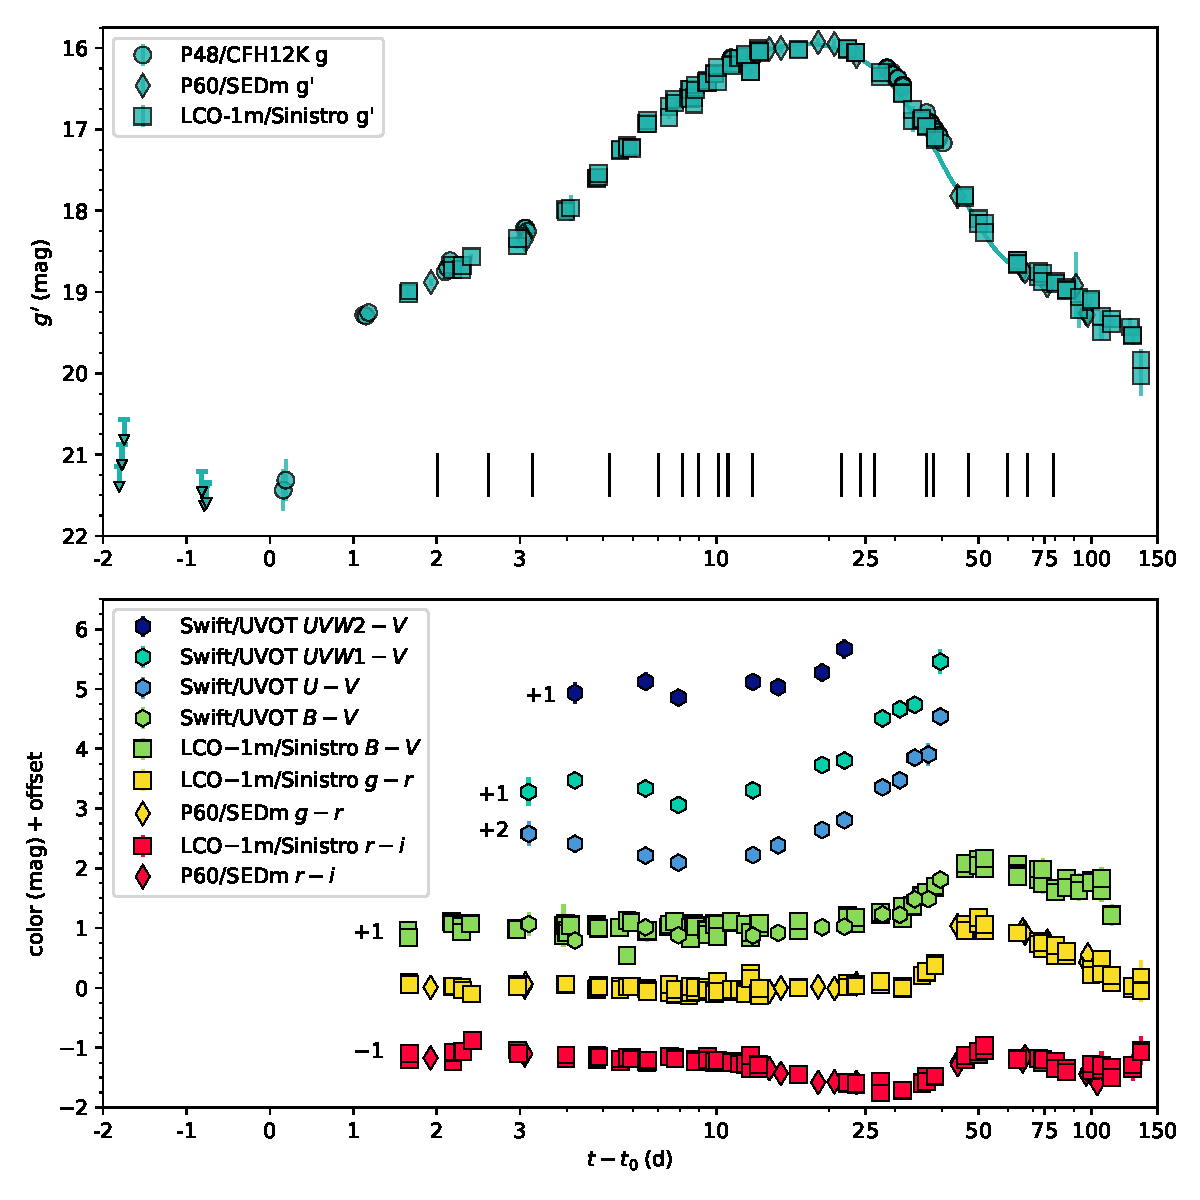
\includegraphics[width=0.95\textwidth]{logLC_with_colors.pdf}
  \caption{Photometric evolution of \abc. \textit{Top}: The $g$-band
  light curve of \abc. Observations from different 
  telescopes are shown with different symbols. Time is measured in 
  rest-frame d relative to the time of first light, $t_0$ (see 
  \S\ref{sec:lc_fit}). Note that the horizontal axis is shown with a linear scale 
  for $-2 \; \mathrm{d} \le t - t_0 \le 3 \; \mathrm{d}$ and a 
  $\log$ scale for $t - t_0 > 3 \; \mathrm{d}$. The solid curve 
  represents the best-fit model from SALT2 
  (\S\ref{sec:classification}). The black ticks near the
  bottom of the panel show epochs of spectroscopic observations.
  \textit{Bottom}: Color curves of \abc. Each color curve is 
  represented with a different color, with each symbol corresponding 
  to a different instrument, as detailed in the legend. Magnitude 
  offsets applied to each color curve are also shown.
  }
  \label{fig:lightcurve}
\end{figure*}

During the spring of 2016, the iPTF survey observed the field of \abc\ every night in either the $g_\mathrm{PTF}$- or 
$R_\mathrm{PTF}$-band.\footnote{P48 observations of \abc\ is reported in the $g_\mathrm{PTF}$ and $R_\mathrm{PTF}$ filters throughout, which are similar to the SDSS $g'$ and $r'$ filters, respectively (see \citealt{2012PASP..124..854O} for details on PTF calibration). The correction from the $g_\mathrm{PTF}$ and $R_\mathrm{PTF}$ filters to SDSS $g'$ and $r'$ requires knowledge of the intrinsic source color (see Eqns.~1 and 2 in \citealt{2012PASP..124..854O}). The spectral diversity of SNe Ia in the days after explosion is poorly constrained, and as a result the color terms for \abc\ at these epochs are unknown. We proceed by assuming $g_\mathrm{PTF}$ and $R_\mathrm{PTF}$ calibration is on the AB system, which strictly speaking is incorrect, but this does not fundamentally alter any of our conclusions.} 
Survey observations were conducted with the
CFH12K camera \citep{2000SPIE.3965...58S} on the Palomar Observatory 
48-inch telescope (P48). Images were processed by the IPAC image
subtraction and discovery pipeline which subtracts off the background
galaxy light with stacked pre-SN images and performs forced
point-spread-function (PSF) photometry at the location of the SN 
\citep{2017PASP..129a4002M}. The
photometry is then calibrated to the PTF photometric catalog
\citep{2012PASP..124..854O}.

After discovery, photometric observations in the $g'$, $r'$ and $i'$
filters were obtained with the SED Machine 
(SEDm; Blagorodnova et al.\ 2017, in prep.) mounted on the Palomar Observatory 
60-inch telescope (P60). We utilized the Fremling Automated Pipeline \citep{2016A&A...593A..68F} to subtract galaxy light from the SEDm images using archival Sloan Digital Sky Survey (SDSS) images as a reference. This pipeline then performed forced-PSF photometry at the location of \abc, which is calibrated to the SDSS catalog \citep{2014ApJS..211...17A}.

Photometric observations in the \textit{BVg'r'i'} filters were conducted by the Las Cambres Observatory (LCO) 1-m
telescope network.  PSF photometry was measured on these images using
the \texttt{lcogtsnpipe} pipeline \citep{2016MNRAS.459.3939V}. The
\textit{BV} magnitudes are calibrated to the Fourth USNO CCD
Astrograph Catalog \citep{2013AJ....145...44Z}, and the \textit{g'r'i'}
magnitudes are calibrated to SDSS Data Release 6
\citep{2008ApJS..175..297A}.

The \textit{Swift} satellite observed \abc\ on 14 epochs, beginning 
$\sim$15 d pre-maximum light through $\sim$22 d post maximum. The SN 
flux is measured via aperture photometry on Ultraviolet-Optical
Telescope (UVOT) images via the usual procedures in 
\texttt{HEASoft}, including corrections for the coincident loss and 
aperture loss. The image counts
are converted to physical fluxes using the latest calibration
\citep{2011AIPC.1358..373B}. There are no pre-SN UVOT images at the 
SN location in the \textit{Swift} archive.  Visual inspection of the
UVOT images suggests negligible host-galaxy contamination in our 
UVOT flux measurements. No X-ray emission is detected from \abc\ by the \textit{Swift} X-ray Telescope (XRT).

The $g$-band discovery data and color curves of \abc\ are 
illustrated in Figure~\ref{fig:lightcurve}.  For convenience, 
magnitudes in 
\textit{all} filters are in the AB system with a zero point of 
$3631$\,Jy. As previously noted the color terms necessary to convert the $g_\mathrm{PTF}$ and $R_\mathrm{PTF}$ to the AB system are unknown and assumed to be zero.

Spectroscopic observations of \abc\ were taken with a variety
of telescopes and instruments over multiple epochs spanning from a
couple of days after explosion to two months after $B$-band maximum. 
An observing log is listed in Table \ref{tab:spec_obs_log}. The spectra were reduced using standard routines in \texttt{IDL}/\texttt{Python}. The optical
spectral evolution of \abc\ is illustrated in Figure
\ref{fig:spec_seq}, which excludes high-resolution Very Large Telescope (VLT) spectra for clarity.

\begin{deluxetable*}{cccccc}
  \tablecaption{Spectroscopic observations of \abc\ \label{tab:spec_obs_log}}
  \tablehead{
    \colhead{Observation MJD} & \colhead{SN phase} & \colhead{Telescope} &
    \colhead{Instrument} & \colhead{Wavelength Coverage (\AA)}
  }
  \startdata
  $57483.26$ & $-16.4$ & DCT & DeVeny\tablenotemark{1} & $3301$--$7499$ \\
  $57483.88$ & $-15.8$ & Gemini-North & GMOS\tablenotemark{2} & $3800$--$9200$ \\
  $57484.51$ & $-15.1$ & Keck-II & DEIMOS\tablenotemark{3} & $5500$--$8099$ \\
  $57486.51$ & $-13.1$ & Keck-II & DEIMOS\tablenotemark{3} & $5500$--$8099$ \\
  $57488.38$ & $-11.3$ & Keck-I & LRIS\tablenotemark{4} & $3055$--$10411$ \\
  $57489.51$ & $-10.1$ & LCOGT-2m & FLOYDS\tablenotemark{5} & $3301$--$8999$ \\
  $57490.40$ & $ -9.3$ & LCOGT-2m & FLOYDS\tablenotemark{5} & $3301$--$9999$ \\
  $57491.55$ & $ -8.1$ & LCOGT-2m & FLOYDS\tablenotemark{5} & $3300$--$9998$ \\
  $57492.20$ & $ -7.5$ & VLT & X-shooter\tablenotemark{6} & $3300$--$24550$ \\
  $57494.00$ & $ -5.7$ & VLT & UVES\tablenotemark{7} & \\
  $57503.32$ & $ +3.7$ & LCOGT-2m & FLOYDS\tablenotemark{5} & $3300$--$9999$ \\
  $57506.00$ & $ +6.3$ & NOT & ALFOSC\tablenotemark{8} & $3602$--$8098$ \\
  $57508.27$ & $ +8.6$ & LCOGT-2m & FLOYDS\tablenotemark{5} & $3301$--$9999$ \\
  $57518.42$ & $+18.8$ & Keck-I & LRIS\tablenotemark{4} & $3071$--$10208$ \\
  $57520.03$ & $+20.4$ & VLT & X-shooter\tablenotemark{6} & $3300$--$24789$ \\
  $57529.40$ & $+29.8$ & LCOGT-2m & FLOYDS\tablenotemark{5} & $4000$--$8998$ \\
  $57542.41$ & $+42.8$ & LCOGT-2m & FLOYDS\tablenotemark{5} & $4000$--$8998$ \\
  $57550.40$ & $+50.8$ & LCOGT-2m & FLOYDS\tablenotemark{5} & $4001$--$8999$ \\
  $57562.38$ & $+62.7$ & LCOGT-2m & FLOYDS\tablenotemark{5} & $4800$--$9300$ \\
  \enddata
  \tablenotetext{1}{The Deveny Spectrograph \citep{2014SPIE.9147E..2NB}}
  \tablenotetext{2}{The Gemini Multi-Object Spectrograph \citep{2004PASP..116..425H}}
  \tablenotetext{3}{DEep Imaging Multi-Object Spectrograph \citep{2003SPIE.4841.1657F}}
  \tablenotetext{4}{Low-Resolution Imaging Spectrometer \citep{1995PASP..107..375O}}
  \tablenotetext{5}{FLOYDS \url{https://lco.global/observatory/instruments/floyds}}
  \tablenotetext{6}{X-shooter \citep{XShooter}}
  \tablenotetext{7}{Ultraviolet and Visual Echelle Spectrograph \citep{2000SPIE.4008..534D}}
  \tablenotetext{8}{The Andalucia Faint Object Spectrograph and Camera \url{http://www.not.iac.es/instruments/alfosc}}
\end{deluxetable*}

\begin{figure*}[!htb]
  \centering
  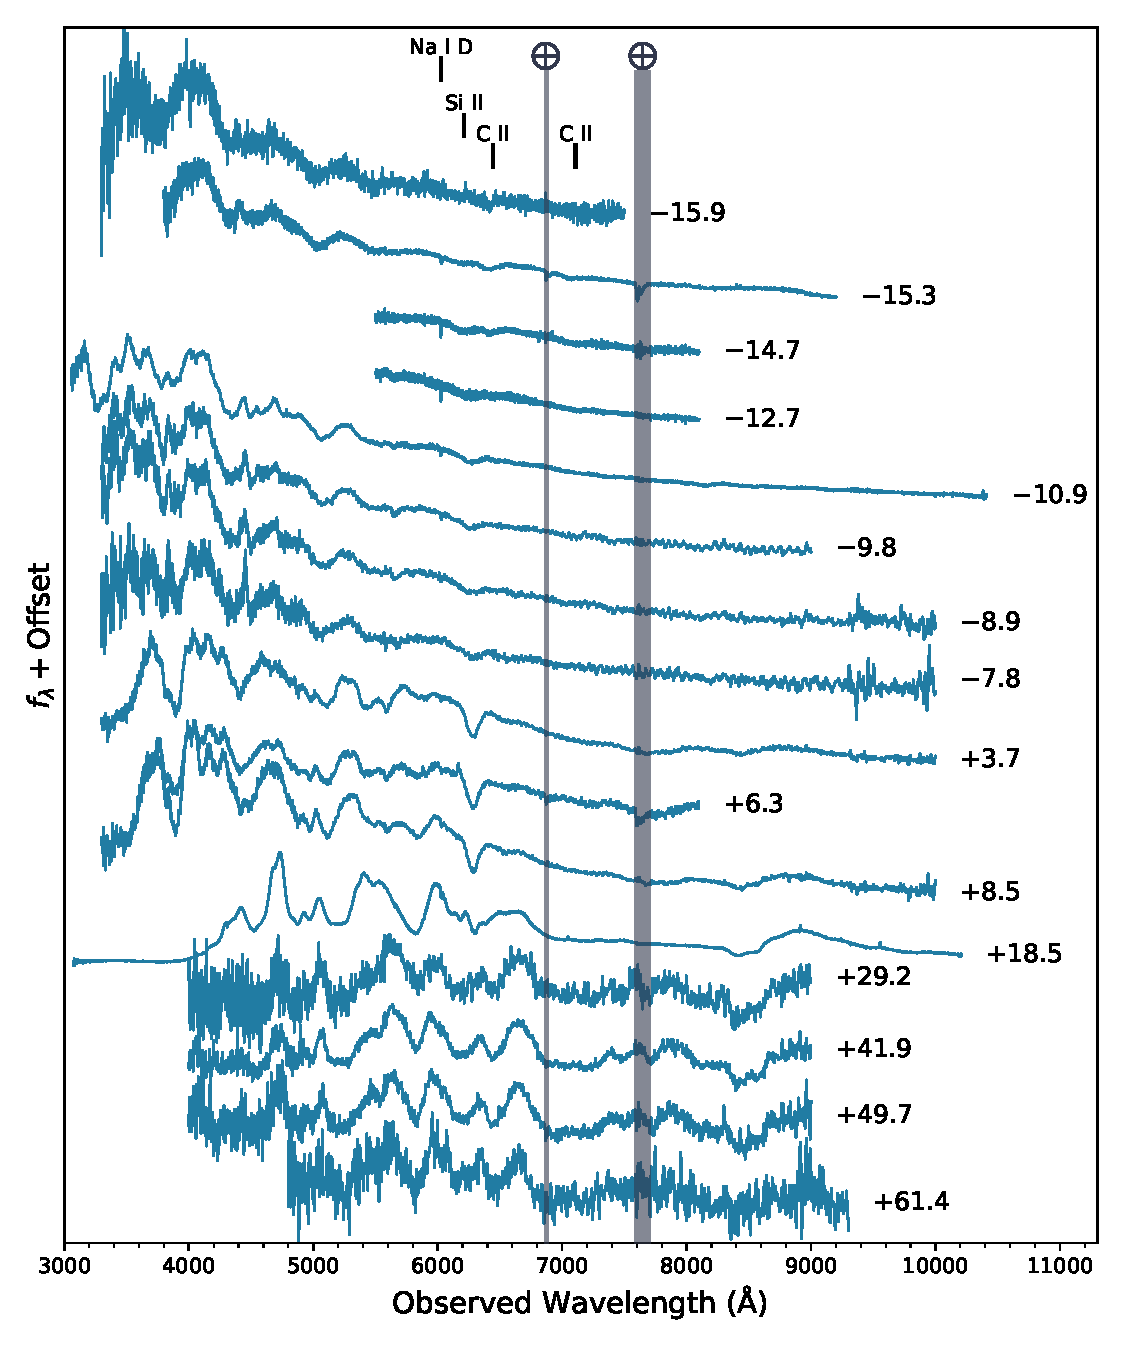
\includegraphics[width=1.0\textwidth]{spectra.pdf}
  \caption{Observed spectral sequence of \abc. For clarity, offsets 
  have been applied to each 
  spectrum which are normalized by their median flux between 
  6,000 and 7,000$\,\textrm{\AA}$. The phase of each spectrum 
  relative to $T_{B_\mathrm{max}}$ is shown. Telluric absorption
  bands are grayed out. The narrow \ion{Na}{1}\,D absorption is also
  highlighted in orange.}
  \label{fig:spec_seq}
\end{figure*}


\section{Reddening, Classification and Host Galaxy}
\label{sec:usual_staff}

\subsection{Reddening}
\label{sec:reddening}

A detailed study of the reddening towards \abc\ is presented in a 
companion paper (Ferretti et al.\ 2017, submitted). Briefly, the 
foreground Galactic extinction toward \abc\
is $E(B-V) = 0.0279 \, \mathrm{mag}$ \citep{2011ApJ...737..103S}. The high-resolution spectra presented in Ferretti et al.\ (2017) show multiple absorption components for both the \ion{Ca}{2}\,H$+$K and \ion{Na}{1}\,D doublets. While the equivalent width (EW) of these lines is quite large, implying a large amount of extinction (e.g., \citealt{2012MNRAS.426.1465P}), Ferretti et al.\ compare the evolution of \abc\ to the well-observed normal type Ia SN\,2011fe and find evidence for only a small amount of extinction. The empirical relation between the EW of \ion{Na}{1}\,D and extinction is known to have a large scatter, and thus, we instead adopt $E(B-V) = 0.05 \, \mathrm{mag}$ as the local extinction for \abc\ (Ferretti et al.\ 2017). For the remainder of our analysis we therefore adopt a total, Galactic $+$ host galaxy, line-of-sight extinction of $E(B-V) = 0.0779 \, \mathrm{mag}$.

\subsection{Classification}
\label{sec:classification}

Using the Supernova Identification (SNID; \citealt{2007ApJ...666.1024B}) package, 
we find the low-resolution spectrum of \abc\ at $+18.8$ d is best matched by normal SNe Ia. Several characteristic features of a SN
Ia, such as \ion{Si}{2}, \ion{S}{2}, can be easily identified in the
spectra of \abc\ (Figure \ref{fig:spec_seq}).

To determine the brightness and time of $B$-band maximum for 
\abc, we fit the P60 light curves with the \texttt{sncosmo} software package.\footnote{The
  \texttt{sncosmo} Python module is available at
  \url{https://sncosmo.readthedocs.io/en/v1.5.x/}.} This fit includes a SALT2 template \citep{2007A&A...466...11G} modified by the line-of-sight extinction
curve \citep{1999PASP..111...63F} with $E(B-V)$ values from 
\S\ref{sec:reddening} and $R_V=3.1$.

We determine the time of rest-frame \textit{B}-band maximum to be 
 $\textrm{MJD}_{max}=57499.54\pm0.23$, the coefficient
of the zeroth principle component $x_0 = 0.0086 \pm 0.0003$, the
coefficient of the first principle component $x_1 = 0.96 \pm 0.15$, 
and the color term $c = 0.033 \pm 0.029$. The best-fit model also 
gives an unreddened apparent peak magnitude of $m^*_{B}=15.80 \pm 
0.04 \,\textrm{mag}$ in the SN rest frame.

For convenience, in the following sections, we define the best-fit
value $\textrm{MJD}_{max}=57499.54$ as the time of $B$-band maximum, $T_{B_\mathrm{max}}$, which we also adopt as phase $t=0$.

\subsection{Host Galaxy}
\label{sec:host}

After establishing \abc\ as a normal SN Ia, we use the latest
calibration \citep{2014A&A...568A..22B} of the Phillips relation
\citep{1993ApJ...413L.105P} using $m^*_{B}$, $x_1$ and $c$ to derive 
a distance modulus $\mu = 34.88 \pm 0.10 \,\textrm{mag}$ to the SN, 
provided that the host galaxy of \abc\ has a stellar mass less than
$10^{10}\sm$. We note that a more massive host galaxy would result 
in a larger inferred distance modulus that is nevertheless 
consistent within the uncertainties.

The location of \abc\ is spatially coincident with a tidal tail of
galaxy NGC\,5221. \citet{2007A&A...465...71T} derived a distance
modulus of $35.0\pm0.4\,\textrm{mag}$ to NGC\,5221 from the 
Tully-Fisher relation, which is consistent with that of \abc.

Separately, \citet{2015MNRAS.447.1531C} observe the 21-cm line in
NGC\,5221 and measure a redshift of $0.0234$, which we adopt for the remaining analysis in this paper.

\section{First Light And Explosion Time}
\label{sec:first_light}

\subsection{Light Curve Fit}
\label{sec:lc_fit}

The time of first light for SNe is usually estimated by 
extrapolating early-phase light curves to determine when the 
SN is equal to 0. Assuming an ideal expanding fireball with 
constant temperature, \citet{1982ApJ...253..785A} derives that $f 
\propto t^2$, where $f$ is the SN flux and $t$ is the time since 
explosion. Despite the basic assumption of a constant temperature at 
early times, multiple studies have found that the early emission 
from type Ia SNe can be described as a power law in time, with 
power-law index consistent with 2, i.e. $f \propto t^2$ (e.g., \citep{2006AJ....132.1707C, 2010ApJ...712..350H, 2011MNRAS.416.2607G}).

As our observations include especially early observations of \abc, there are upper limits $\sim$1 d prior to the discovery epoch, we model the early flux from \abc\ as a power law, but allow the power-lax index to vary, as opposed to fixing it at 2, to account for potential variations in the photospheric temperature during expansion:
\begin{equation}
  \label{eq:broken_power_law}
  f(t) \left\{
    \begin{array}{ll}
      = 0,\ \textrm{when}\ t<t_0 \\
      \propto (t-t_0)^{\alpha},\ \textrm{when}\ t>t_0
    \end{array}
  \right.\ ,
\end{equation}
where $t_0$ is the time of first light, $\alpha$ is the power-law index, and $t$ is measured in the rest-frame of the SN. To determine $t_0$ and $\alpha$ we fit the earliest observations of \abc. Due to slight variations in the passbands, we fit the model to the relative flux measured in the $g_\mathrm{PTF}$-band, which is the only filter with observations prior to first light, a necessity for constraining $t_0$. 

To determine the best fit parameters, we search a large grid over $t_0$, $\alpha$
and the proportionality constant, and minimize $\chi^2$. 
The modeling results show that the SN flux rises approximately
linearly between
$t=-18\,\textrm{d}$ and $t=-14\,\textrm{d}$. Figure \ref{fig:early_lc_fit} shows the best-fit result and
the joint marginal distribution of $t_0$ and $\alpha$. From the
best-fit model we obtain $\alpha=0.98 \pm ^{0.16}_{0.14}$ and $t_0=-17.91 \pm ^{0.07}_{0.15}$ d, where the uncertainties represent the marginalized 95\% confidence intervals. Our first
detection of \abc\ occurred $\sim{0.15}\,\textrm{d}$ after 
the SN first light. Figure~\ref{fig:early_lc_fit} additionally shows $g'$-bands observations from P60 and LCO, where we have normalized the flux assuming that the $g$ magnitudes from each instrument have the same zero-point. This assumption is incorrect (see \S\ref{sec:obs}), and, as expected, the residuals show a systematic offset between the $g_\mathrm{PTF}$-band and the $g'$-band. Nevertheless, if we ignore this systematic and fit all of the $g$-band observations simultaneous we obtain marginalized best-fit parameters that are consistent within the uncertainties with the $g_\mathrm{PTF}$-only values above. In the analysis that follows, the precise values of the best-fit parameters is not important. The critical finding here is that $\alpha \approx 1$ and $t_0 \approx -18 \, \mathrm{d}$. 

\begin{figure*}[!htb]
  \centering
  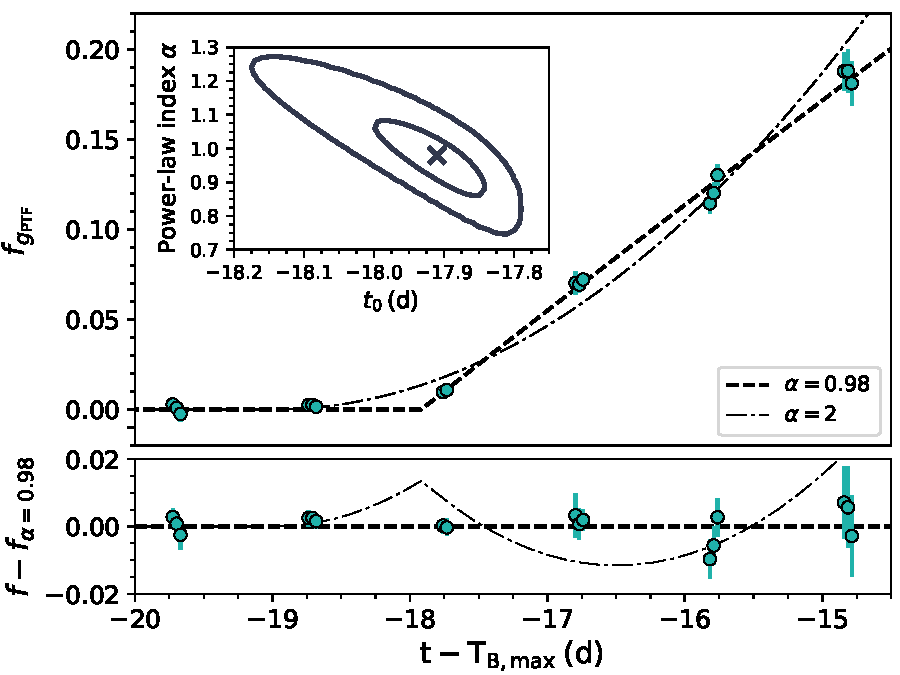
\includegraphics[width=0.95\textwidth]{early_lc.pdf}
  \caption{Best-fit power-law model to describe the early flux from 
  \abc\ in the $g_\mathrm{PTF}$-band. The model flux, adopting 
  best-fit parameters $\alpha=0.98$ and $t_0=-17.94\,\textrm{d}$, 
  is shown as a solid black line in the top panel. The lower panel 
  shows the model residuals, and the symbols are the same as in
  Figure~\ref{fig:lightcurve}. The model is fit to just the 
  $g_\mathrm{PTF}$-band observations to avoid systematic difference 
  between the filters (see the text for further 
  details). The joint distribution of $t_0$ and $\alpha$ is 
  illustrated in the inset of the upper panel. The solid and 
  dashed contours represent the $68\%$ and $99.7\%$ confidence 
  levels.
  }
  \label{fig:early_lc_fit}
\end{figure*}

% Starting around $t=-15\,\textrm{d}$, the $g$-band light curve
% deviates from the above best-fit model and
% rises significantly faster, indicating a
% change in the power-law index $\alpha$. In fact, between $t=-14\,\mathrm{d}$ and $t=-8\,\mathrm{d}$ the light curve is well fit by a power law of index $1.40$. In other words, the entire light curve
% before $t=-8$\,days can be approximated by a broken power-law model
% (e.g.,
% \citealt{2016arXiv161202097Z,
%   2016arXiv161202725Z}).

As previously noted, the early emission from most SNe Ia can be explained via a $f \propto t^2$ model, including SNe with extremely early observations like \abc, such as SN\,2011fe \citep{2011Natur.480..344N}. Thus, the near-linear rise in flux over the first few days after first light for \abc\ is unusual. To our knowledge this behavior has only been observed in 2 other SNe (2013dy, 2014J; \citealt{2013ApJ...778L..15Z,2014ApJ...783L..24Z}). Any model to explain the observations of \abc\ must be able to account for this unusual behavior in the days after first light.  

\subsection{Expansion Velocity Fit}
\label{sec:early_vel}

As previously noted, $t_0$ does not correspond to the time of 
explosion, $t_\mathrm{exp}$, for type Ia SNe as the SN may 
experience a dark phase following shock breakout before radioactive 
energy can diffuse to the photosphere. \citet{2014ApJ...784...85P} 
instead suggest that measurements of the photospheric velocity be 
used to determine $t_\mathrm{exp}$ given that the ejecta begin 
expanding from the moment of explosion.  Assuming a
constant opacity in the ejecta, \citeauthor{2014ApJ...784...85P} 
find that the photospheric velocity evolves as
$v_{ph}\propto(t-t_{exp})^{-0.22}$. While the photospheric velocity
is not easy to measure, line velocities of \ion{Si}{2} or \ion{Ca}{2}
can be used as a proxy
\citep{2014ApJ...784...85P,2016ApJ...826..144S}.

In the case of \abc, the \ion{Ca}{2} IR triplet is very weak, 
likely due to high temperatures in the ejecta. Thus, we
determine the photospheric velocity from the 
\ion{Si}{2}\,$\lambda$6355 line. Visual inspection shows no 
sign of multi-velocity components of \ion{Si}{2}, and that 
\ion{C}{2}\,$\lambda$6580 line overlaps the red
wing of the \ion{Si}{2} line (see Figures~\ref{fig:spec_seq} and \ref{fig:carbon}). Consequently, we model the observed 
spectra between 5,900 and 6,500\,\AA (rest-frame) as the combination 
of two gaussian kernels plus a linear baseline, which
accounts for \ion{Si}{2}, \ion{C}{2} and the
continuum, respectively. The expansion
velocity of \ion{Si}{2} is measured by the central wavelength
of the \ion{Si}{2} Gaussian kernel.

\begin{figure*}[!thb]
  \centering
  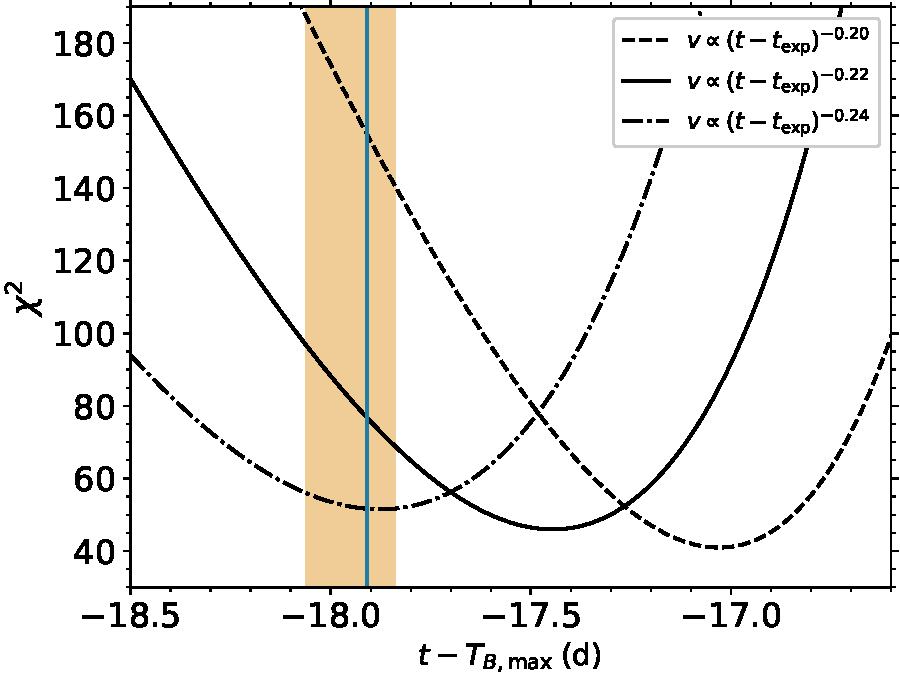
\includegraphics[width=0.45\textwidth]{Chi2.pdf}
  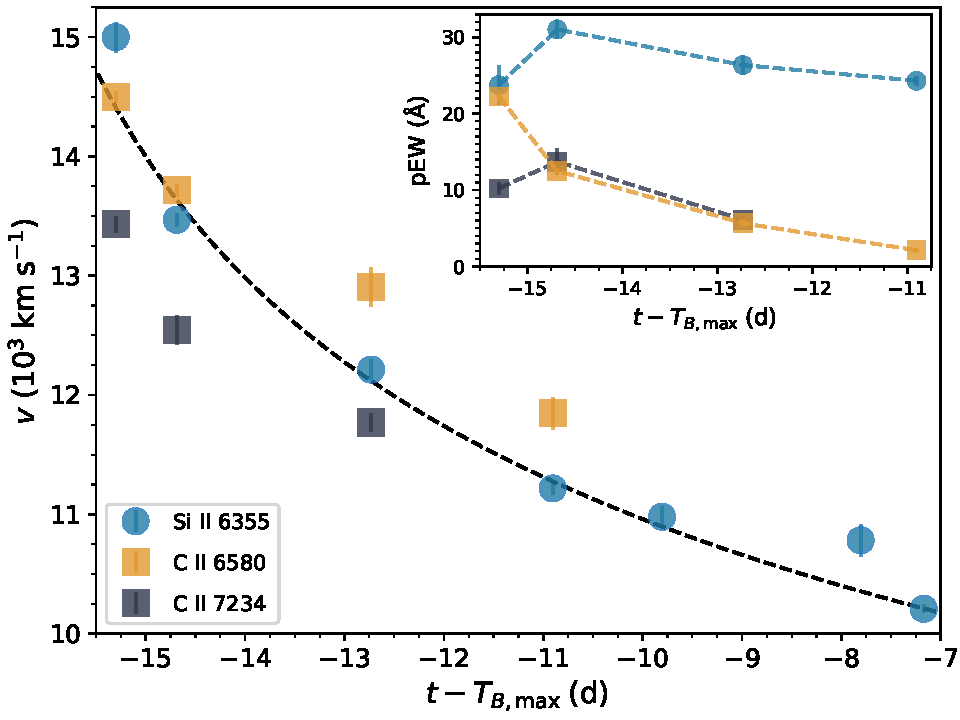
\includegraphics[width=0.45\textwidth]{VelocityPlot.pdf}
  \caption{Constraints on $t_{exp}$ from fitting the velocity
    evolution of \ion{Si}{2}.
    \textit{Left panel:} the dashed, solid
    and dash-dotted curves show $\chi^2$ for fitting power laws with
    indices $-0.20$, $-0.22$ and $-0.24$, respectively. The blue
    vertical line and the orange shaded region indicate $t_0$ and its
    95\% confidence interval from Section
    \ref{sec:lc_fit}, respectively.
    \textit{Right panel:} Observed \ion{Si}{2}\,$\lambda$6355
    velocities (blue circles) and the best-fit power-law model
     with an index of $-0.22$ (dashed line). Additionally the 
     measured velocites of \ion{C}{2}\,$\lambda\lambda$6580, 7234 
     are shown.}
  \label{fig:velocity_t_exp}
\end{figure*}

We fit the measured velocities of \ion{Si}{2}\,$\lambda$6355 to the
$v\propto(t-t_{exp})^{-0.22}$ model by minimizing the $\chi^2$ value and find the best-fit explosion time relative to $T_{B,\mathrm{max}}$ in the SN rest frame to be $t_{exp} = -17.45 \pm ^{0.14}_{0.16}\;\textrm{d}$, where the uncertainties represent the 95\% confidence interval (Figure \ref{fig:velocity_t_exp}). Following the analysis in \citet{2014ApJ...784...85P}, we additionally alter the power-law index to $-0.20$ and $-0.24$ to examine the sensitively of the result on the assumed power-law index. We find that this variation in the power-law index result in inferred explosion times that vary by $\approx$1 d (Figure \ref{fig:velocity_t_exp}). Given the theorhetical expectation that $v \propto t^{-0.22}$, we adopt $t_{exp} = -17.45 \pm 0.5 \; \mathrm{d}$, where the uncertainty reflects possible variations in the power-lax index (see \citealt{2014ApJ...784...85P}).

Comparing our estimates for $t_{exp}$ and $t_0$ (left panel of 
Figure \ref{fig:velocity_t_exp}), we find that 
$t_0\lessapprox t_{exp}$.
Since physical causality requires $t_{exp}<t_0$, we draw the qualitative
conclusion that $t_0\simeq t_{exp}$, which is consistent to within the uncertainties.

% From $t_{exp}$, we estimate the actual rise time of \abc\ from the
% time of explosion to \textit{B}-band maximum to be $17.95$ d.  In
% comparison, SN2011fe has $t_0=-17.7$ d \citep{2013A&A...554A..27P}
% with a preceding dark period of $\sim 1$ day
% \citep{2014ApJ...784...85P}. ASASSN-14lp has $t_0=-16.94$ days with a
% preceding dark period of about acouple of days
% \citep{2016ApJ...826..144S}. This comparison suggests that the actual
% rise time of a SN Ia between the SN explosion and the \textit{B}-band
% maximum is roughly a constant, which largely depends on the total mass
% of synthesized $^{56}$Ni.\ycao{I am not convinced by this last sentence}

\subsection{Strong and Short-Lived Carbon Features}
\label{sec:carbon}

The early spectra of \abc\ exhibit unusually strong absorption due 
to \ion{C}{2} $\lambda\lambda$6580, 7234. We highlight the evolution 
of these spectral features in Figure~\ref{fig:carbon}. From these 
spectra we see that \ion{C}{2}\,$\lambda$6580 is as strong as 
\ion{Si}{2}\,$\lambda$6355 at $t \approx -16 \; \mathrm{d}$. The 
strength of the \ion{C}{2} lines declines with time to the point 
where they are no longer detectible more than 1 wk after explosion.

\begin{figure}[]
  \centering
  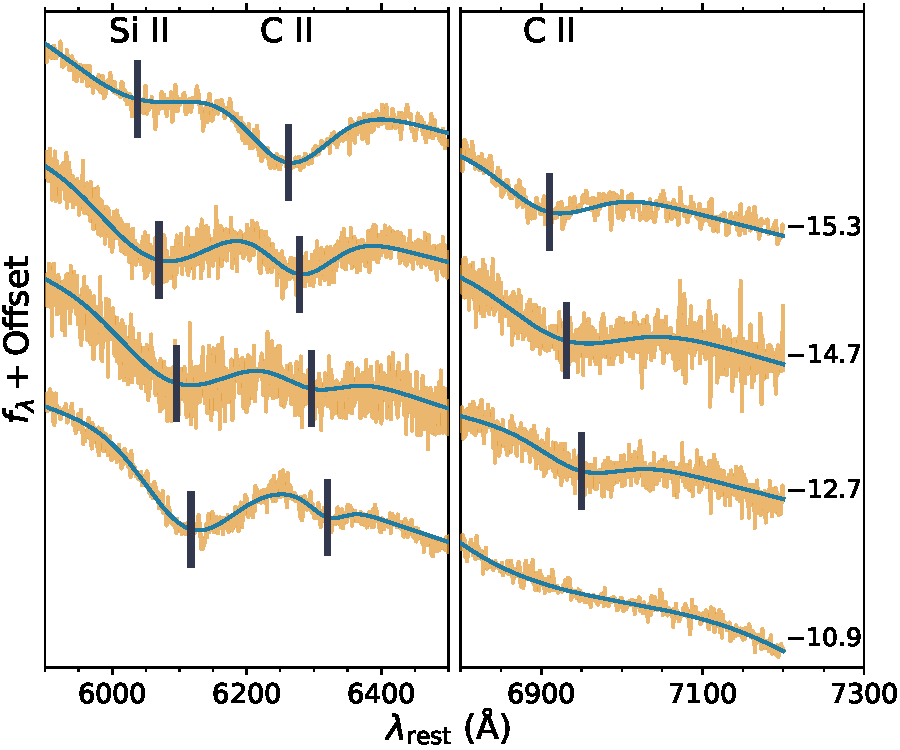
\includegraphics[width=0.49\textwidth]{CarbonFeature.pdf}
  \caption{Evolution of the \ion{C}{2} features observed in the 
  early spectra of \abc. The raw spectra are shown in orange, while 
  the solid blue lines show the best-fit models including gaussian 
  components for each line and a linear component for the continuum 
  (see text for further details). The dark grey vertical lines show 
  the measured line centers, indicating the decline in the 
  photosphere velocity in the $\sim$wk after explosion (note that 
  \ion{C}{2}\,$\lambda$7234 is not detected in the $-10.9$ d 
  spectrum). The phase of each spectrum relative to 
  $T_{B,\mathrm{max}}$ is shown to the right of each spectrum.
  }
  \label{fig:carbon}
\end{figure}

Similar to our analysis of the \ion{Si}{2}\,$\lambda$6355 line, we 
can measure velocities and pseudo-equivalent widths (pEWs) of 
\ion{C}{2}\,$\lambda\lambda$6580, 7234. We compare the velocity 
evolution of the \ion{C}{2} lines to \ion{Si}{2} in the right panel 
of Figure \ref{fig:velocity_t_exp} and the pEW evolution is
shown in Figure \ref{fig:ew}. These measurements confirm the qualitative analysis from Figure~\ref{fig:carbon}: namely, the pEW of \ion{C}{2}\,$\lambda$6580 is comparable to that
of \ion{Si}{2}\,$\lambda$6355 at $t \approx -16 \; \mathrm{d}$ and 
the pEW of \ion{C}{2} 
decreases until the feature is no longer detectable 
around $t=-10$ days.

\begin{figure}[]
  \centering
  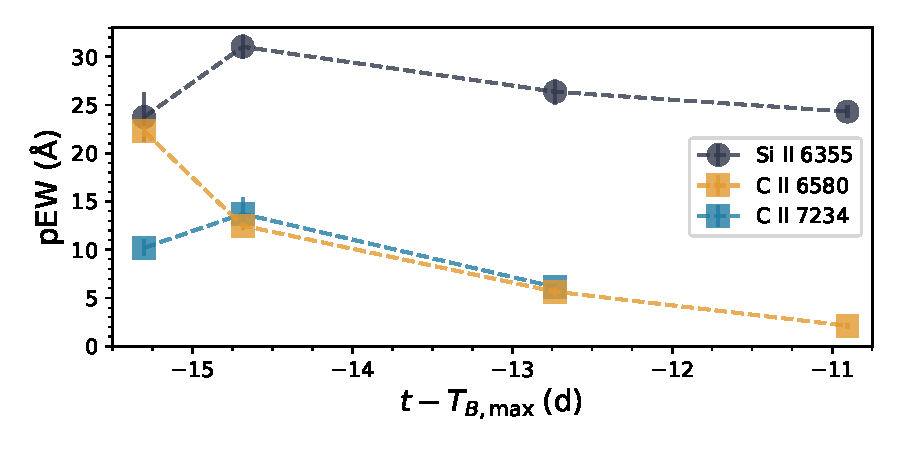
\includegraphics[width=0.45\textwidth]{pEW.pdf}
  \caption{Evolution of the pseudo-equivalent width of 
  \ion{Si}{2}\,$\lambda$6355, and \ion{C}{2}\,$\lambda\lambda$6580, 
  7234 in the week following explosion.}
  \label{fig:ew}
\end{figure}

The detection of \ion{C}{2} in SNe Ia spectra is relatively rare
as it requires both unburned carbon, which is likely only present in the outermost layers of the ejecta, and non-local thermal equilibrium effects in order to excite the ionized carbon (e.g., \citealt{2007ApJ...654L..53T}). Spectra obtained around or after $T_{B_\mathrm{max}}$ rarely show \ion{C}{2} as the photosphere has receded from the outermost ejecta, while pre-max spectra show evidence for \ion{C}{2} in $\sim$1/4 of all normal SNe Ia (e.g., \citealt{2011ApJ...732...30P,2012MNRAS.425.1917S,2011ApJ...743...27T}), but the signatures are typically weak. While we caution that the sample of normal SNe Ia with spectra taken within a few days of explosion is small, SN\,2013dy is the only other object known to have strong \ion{C}{2} features like \abc\ \citet{2013ApJ...778L..15Z}. As a counterexample, SN\,2011fe only exhibited weak \ion{C}{2} features in its first spectra
\citep{2012ApJ...752L..26P}. Thus, models of \abc\ must explain the anomalously strong \ion{C}{2} absorption observed shortly after explosion.


\section{Discussion}
\label{sec:lc_energy}

We have identified several unusual properties in the early observations of \abc, including: (i) a near-linear photometric rise in the days after explosion, (ii) the lack of a dark phase typical of most SNe Ia, and (iii) the presence of strong \ion{C}{2} absorption. While most SNe Ia are powered purely by radioactive decay, the observed radiation shortly after explosion can also include contributions 
from SN shock cooling or the collision of the SN ejecta with a non-degenerate companion. Here we consider those scenarios as a possible explanation for the early behavior of \abc. 

\subsection{SN Shock Cooling}

The shock breakout of a SN Ia lasts for a fraction of a second due to
compact size of the exploding star. Emission from the subsequent 
cooling phase may last for several days, however (e.g., 
\citealt{2010ApJ...708..598P}). Following the analysis of \citet{2012ApJ...744L..17B} for SN\,2011fe, we
compare the early-phase $g_\mathrm{PTF}$ light curve of \abc\ with
two shock cooling models \citep{2011ApJ...728...63R, 
2010ApJ...708..598P}. From this analysis, we constrain the \abc\ 
progenitor radius to be $<1\sr$. Our observations of \abc\ cannot 
place tight constraints on the size of SNe Ia progenitors. Indeed, 
for a typical WD radius, such as that inferred for SN\,2011fe 
($\lesssim 0.02$--$0.04\,\sr$; \citealt{2012ApJ...744L..17B, 
2014ApJ...784...85P}), the expected emission from shock cooling is 
$\sim$2 mag fainter than the P48 $g_\mathrm{PTF}$ detection limit. 
Thus, we conclude that shock cooling does not contribute to the 
early emission from \abc.

\subsection{SN-Companion collision}

The detection of excess emission due to the collision of SN ejecta 
with a non-degenerate companion requires a favorable orbital 
alignment relative to the line of sight. Thus, from geometric 
considerations alone the probability of detecting ejecta-companion 
interaction is low, $\sim$10\%. For any single type Ia SN, this 
probability is further reduced because many explosions come from 
WD-WD binaries. \citet{2010ApJ...708.1025K} calculates that the 
collision of SN ejecta with a companion  
generates thermal emission with a spectrum that peaks in the 
UV. Thus, any resulting \textit{g}-band emission is very weak.

To examine the possibility of a SN-companion signature in the early
light curve of \abc, we employ the \citet{2010ApJ...708.1025K}
model and assume canonical ejecta mass of $1.4\sm$, expansion velocity of
$10^{4}\,\textrm{km}\,\textrm{s}^{-1}$, and constant opacity of
$0.2\,\textrm{cm}^2\,\textrm{g}^{-1}$. We calculate the expected 
$g_\mathrm{PTF}$ brightness of an ejecta-companion collision at the 
distance of \abc\ using the parameterized equations in 
\citet{2012ApJ...749...18B}. If we assume the binary is aligned with 
the optimal orientation relative to the line of sight, the binary 
separation would need to exceed $2\times10^{14}\,\textrm{cm}$ to 
explain the initial detection of \abc. Assuming the companion fills 
its Roche lobe, it would need to 
have a radius of $\sim10^{14}\,\textrm{cm}\simeq10 \,\mathrm{AU}$.
Such a radius is implausibly large for a WD binary companion, 
therefore, we conclude that the early emission from \abc\ is not 
due to a collision between the ejecta and a non-degenerate companion. Our early \textit{Swift} observations support this conclusion, as the UV $-$ optical colors are very red, whereas iPTF\,14atg exhibited much bluer UV $-$ optical colors at the same epoch \citep{2015Natur.521..328C}.

% \begin{figure}[!thb]
%   \centering
%   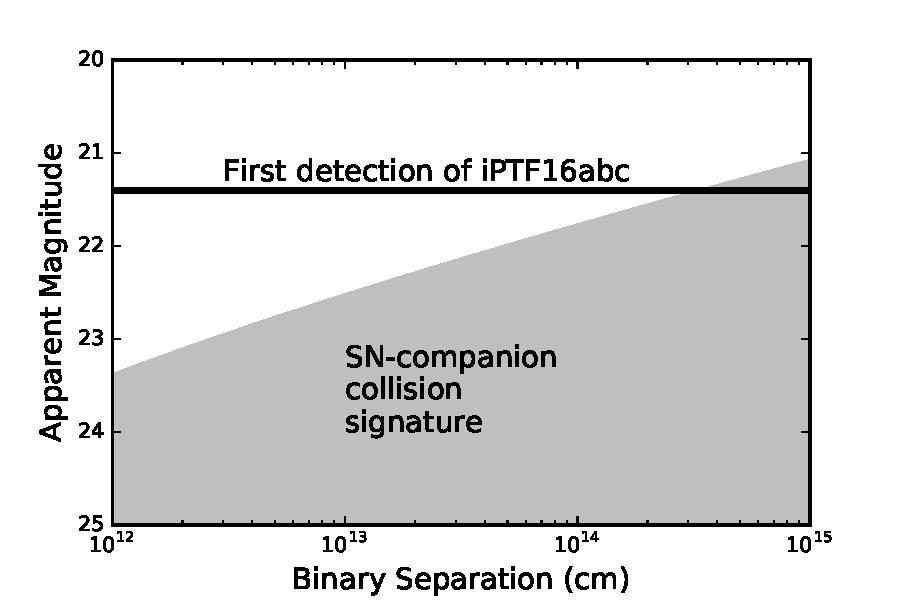
\includegraphics[width=0.45\textwidth]{SNCompanion.pdf}
%   \caption{Apparent magnitude of a SN-companion collision (gray region)
%     against the first detection of \abc\ (black). \amiller{Cut this
%     figure? Doesn't add a lot of information.}}
%   \label{fig:SN-companion}
% \end{figure}

\subsection{Interaction with Diffuse Material}

Here we consider a model that has not, as of yet, been discussed in the context of \abc. In the context of SN\,2011fe, \citet{2014MNRAS.441..532D} recently examined pulsational delayed-detonation (PDD) models as an explanation for some SNe Ia. Briefly, PDD models differ from ``standard'' delayed detonation (DD) models in that the initial deflagration causes the WD to expand resulting in the release of some unbound material. As the bound material contracts, eventually a subsequent detonation occurs.\footnote{\citet{2014MNRAS.441..532D} note that the deflagration and detonation in their PDD models are artificially triggered.} An important consequence of this sequence for PDD models is that they naturally produce material that avoids burning, unlike DD models that typically leave no unburnt material. This enables the presence of significantly more carbon in the outer layers of the SN ejecta \citep{2014MNRAS.441..532D}.

While examining observations of SN\,2011fe in the context of DD models, \citet{2014MNRAS.441..532D} find that the models are universally too faint and red at early times, $\sim$24-48 hr after explosion. These discrepancies can be somewhat improved if the newly synthesized $^{56}$Ni is artificially mixed throughout the SN ejecta (see \S\ref{sec:Ni_mixing} for further details on the importance of mixing). Instead, \citet{2014MNRAS.441..532D} find that PDD models provide a better match to observations. Briefly, the diffuse material surrounding the WD heats the outer layers of the SN ejecta leading to a steeper more luminous rise, with bluer colors in the few days after explosion. Importantly, the PDD models are nearly indistinguishable from DD models around and post peak. 

Qualitatively, the PDD models provide a better match to the observations of \abc\ than DD models. In particular, PDD models provide higher luminosities and faster rise times in the days after explosion, a more rapid evolution towards blue optical colors, and the formation of strong \ion{C}{2} lines that gradually disappear in the $\sim$week after explosion. Quantitatively, there are still some short comings of the models presented in \citet{2014MNRAS.441..532D}. In particular, the power-law index for the $g$-band rise is $\alpha \approx 3$ for each of the PDD models, which is significantly more steep than $\alpha = 0.98$, which we measure for \abc. The optical colors for \abc\ are blue from our first epoch $\sim$1.7 d after explosion and remain approximately constant in the 10 d after explosion, whereas the PDD models in \citet{2014MNRAS.441..532D} either exhibit distinct color evolution (i.e.\ are not constant) or are too red in the first few days after explosion. Nevertheless, the PDD models presented in \citet{2014MNRAS.441..532D} provide several attractive explanations for the unusual features in the early behavior of \abc, and it may be possible that small adjustments to the model, e.g., additional mixing of the radioactive products from the explosion, can better match \abc.

\subsection{Strong $^{56}Ni$ Mixing as an Explanation for \abc}
\label{sec:Ni_mixing}

Having ruled out other possibilities we now consider whether the unusual properties of \abc\ can be explained simply by invoking strong mixing in the SN ejecta. As previously mentioned, strong mixing can lead to a short dark phase and \ion{C}{2} absorption. Here we additionally examine if strong mixing can explain the rapid, near-linear rise in the light curve.

In Figure~\ref{fig:Ni56LC} we compare model calculations from \citet{2016ApJ...826...96P} to the observed photometry of \abc. The \citeauthor{2016ApJ...826...96P} models employ a piston driven explosion to explode a single WD progenitor model. As the piston explosion does not result in any nucleosynthesis, the distribution of $^{56}$Ni in the ejecta must be prescribed by hand, which enables their study of the effects of mixing on the resulting SN emission. Each model employs a fixed $0.5\,\sm$ of $^{56}$Ni that has been distributed throughout the ejecta via boxcar averaging (see their Figure~1). The resulting light curves are synthesized using the SuperNova Explosion Code (\texttt{SNEC}; \citealt{2015ApJ...814...63M}), as shown in Figure~\ref{fig:Ni56LC}. Broadly speaking, the results can be summarized as follows: SN with strong mixing exhibit a rapid almost linear rise and quickly develop blue colors, whereas models where the $^{56}$Ni is confined to the innermost layers of the ejecta remain very faint for days after explosion while exhibiting relatively red optical colors during this period. The fast rise and blue color of \abc\ are consistent with the strong mixing models from \citet{2016ApJ...826...96P}, as shown in Figure~\ref{fig:Ni56LC}. We conclude that the early observations of \abc\ can be explained if the $^{56}$Ni synthesized in the explosion is mixed into the outermost layers of the SN ejecta. 

\begin{figure}[]
  \centering
  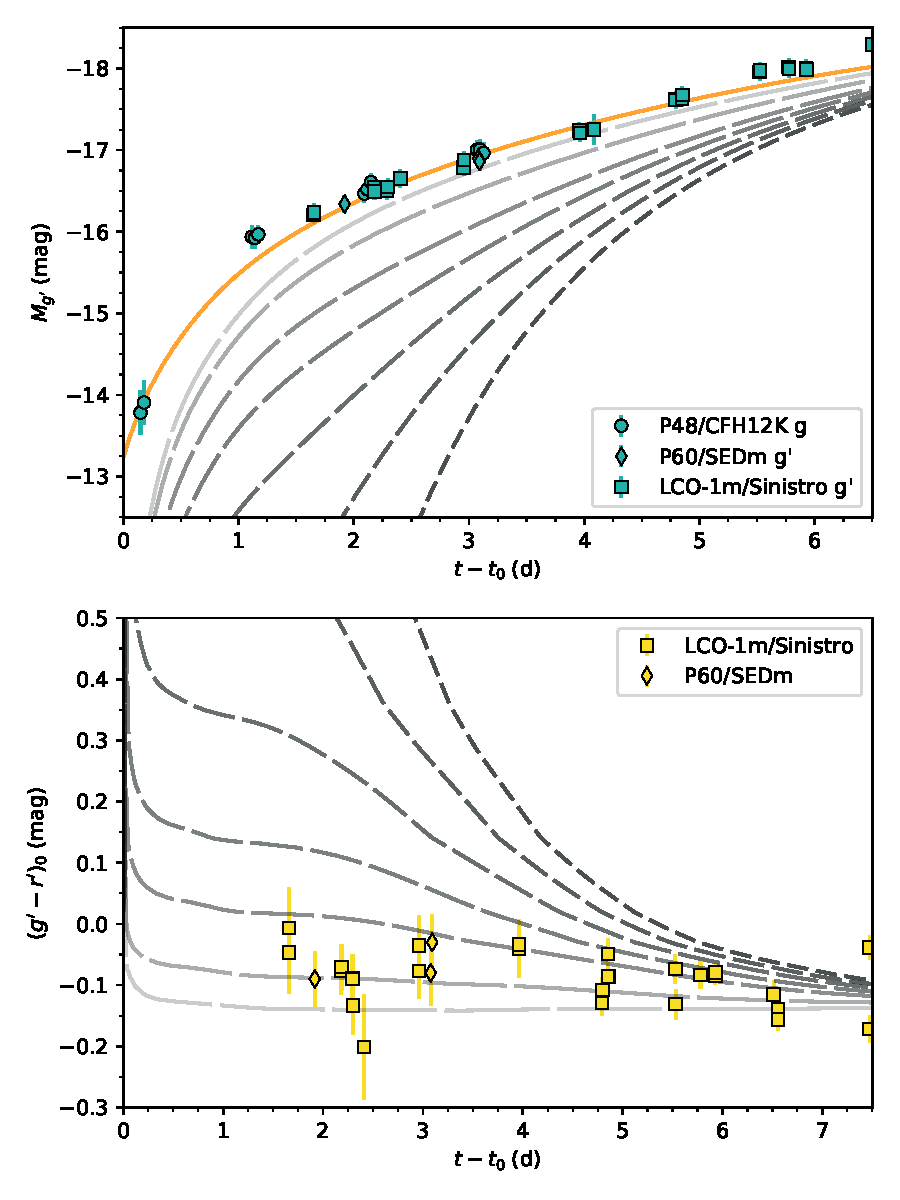
\includegraphics[width=0.48\textwidth]{iPTF16abc_Ni_lc.pdf}
  \caption{Photometric comparison of \abc\ and the theoretical 
  models of \citet{2016ApJ...826...96P}. The amount of $^{56}$Ni 
  mixing in the SN ejecta increases from the short-dash, dark lines 
  to the long-dash, light lines.
  \textit{Top}: $M_g$ vs.\ time, where the observed $g$-band 
  magnitudes  
  have been corrected to $M_g$ using the distance modulus to \abc\ 
  (\S\ref{sec:host})
  and the total line-of-site reddening ($E(B-V) = 0.078 \; 
  \mathrm{mag}$; Ferretti et al.\ 2017, submitted).
  \textit{Bottom}: $(g' - r')_0$ vs.\ time. The observed colors have 
  been corrected for reddening.
  }
  \label{fig:Ni56LC}
\end{figure}


\section{Conclusion}
\label{sec:conclusion}

We have presented observations of the extraordinarily early discovery of the 
normal Type Ia supernova \abc. Our fast-response follow-up 
campaign allowed us to draw the following conclusions:

\begin{itemize}
    \item Extrapolation of the early light curve shows that the initial detection of \abc\ occurred only $\sim$0.2 d after the time of first light.

    \item The early emission from \abc\ is powered solely by radioactive $^{56}$Ni decay. We find no evidence for detectable signatures of SN shock cooling or the collision of the SN ejecta with a non-degnerate binary companion.

\item The velocity evolution of the SN ejecta shows that the time of explosion is approximately equal to the time of first light. This constitutes the first major piece of evidence that $^{56}$Ni is strongly mixed into the outer layers of the supernova ejecta.

\item The strong and short-lived carbon features seen in the 
earliest spectra of \abc\ can only be explained if there is incomplete burning during the explosion and there is a non-thermal 
radiation source in the outermost layers of the ejecta to excite the ionized carbon. $^{56}$Ni decay is the likely source of the non-thermal emission, providing another piece of evidence for strong mixing in the ejecta of \abc. 

\textbf{Does anyone know of any theoretical studies that specifically predict incomplete burning and strong Ni mixing?}

\item Finally, we show that the early light curve evolution and colors of \abc\ are well matched by the theoretical models of \citet{2016ApJ...826...96P} that include significant mixing of $^{56}$Ni into the outer layers of the SN ejecta. 
 
\end{itemize}
%
Taken together, these observations all indicate that the nucleosynthetic products from the explosion are well mixed throughout the SN ejecta. There are elements of the PDD models from \citet{2014MNRAS.441..532D} that are attractive for explaining \abc, in particular, the strong \ion{C}{2} absorption seen at early times. In the future, it would be useful to investigate PDD models that incorporate strong $^{56}Ni$ mixing to see if they better replicate the observations of \abc.  

Extremely early observations of young SNe provide a ``smoking
gun'' to probe the mixing level in the ejecta, which, in turn, is 
a result of the explosion mechanism. Wide-field, high-cadence surveys, such as the Zwicky Transient Facility \citep{2016PASP..128h4501B} and ATLAS \citep{2011PASP..123...58T,2013RSPTA.37120269T}, will discover a large number of very young supernovae over the next few years. These surveys will generate large observational samples that probe SNe in the hours after explosion. While the sample of extremely young SNe Ia will grow by more than an order of magnitude, the detection of shock breakout cooling and ejecta-companion interaction will prove challenging. Given the diminutive size of WDs, the thermal emission following shock breakout can only be detected to $\sim 10\,\mathrm{Mpc}$ on 1-m class telescopes. Furthermore, only $\sim$10\% of single-degenerate progenitors are expected to give rise to detectable emission following the collision of the SN ejecta with the binary companion \citep{2010ApJ...708.1025K}. Despite these limitations, this study of \abc\ shows that the early detection of SNe Ia can constrain the explosion physics by probing the amount of mixing in the SN ejecta. Moving forward, a large sample of such objects will enable strict constraints on the proposed explosion mechanisms for type Ia SNe.

Finally, we close by emphasizing the importance of fast-response photometric and spectroscopic follow-up campaigns. Without the early recognition of the youth of this SN and the associated follow-up, much of the analysis presented herein would not have been possible. The ability to trigger such observations is essential to improve our understanding of the physics of SNe Ia.

\acknowledgements

We are deeply grateful to R.~C.~Thomas for induldging a slew of questions regarding \ion{C}{2} in SNe. Similarly, it is our pleasure to buy a beer for R.~Amanullah and U.~Feindt for discussions regarding SALT2. 

Much of the analysis presented herein would not have been possible without the help of several observers. We thank M.~West for taking the first spectrum of \abc\ as a ToO on the DCT. We also thank the Gemini service observers for executing our ToO observations. Additionally, J.~Cohen, N.~Suzuki, V.~Ravi, R.~Walters, A.~Ho, and L.~Yan helped obtain data for this paper.

% Observers:  Plant,J.Torres,Jang,Cunningham,Guhathakurta, Vedantham, De

AAM is funded by the Large Synoptic Survey Telescope Corporation in support of the Data Science Fellowship Program. YC thanks support from a postdoc fellowship in the eScience institute, University of Washington.

DAH, CM, and GH are supported by NSF-1313484. Support for IA was provided by NASA through the Einstein Fellowship Program, grant PF6-170148.

The Intermediate Palomar Transient Factory project is a scientific collaboration among the California Institute of Technology, Los Alamos National Laboratory, the University of Wisconsin, Milwaukee, the Oskar Klein Center, the Weizmann Institute of Science, the TANGO Program of the University System of Taiwan, and the Kavli Institute for the Physics and Mathematics of the Universe. This work was supported by the GROWTH project funded by the National Science Foundation under Grant No 1545949. Part of this research was carried out at the Jet Propulsion Laboratory, California Institute of Technology, under a contract with the NASA. This work makes use of observations from the LCO network.


\bibliographystyle{aasjournal}
\bibliography{ref}

\end{document}
